\documentclass[12pt,a4paper]{report}

%\includeonly{cover/cimlap, chapters/1_introduction}

\usepackage{styles/dolgozat}

% programkód beillesztéséhez
\usepackage{listings}
% listing float neve
\renewcommand{\lstlistingname}{Programkód}
%\renewcommand{\lstlistlistingname}{Programkódok listája}
%saját listings style-ok, és a style-t használó parancsok definíciói
\usepackage{styles/cpp}
\usepackage{styles/python}
%\usepackage{styles/java}
%\usepackage{styles/rust}

%% egyéb csomagok betöltése itt, vagy a dolgozat.sty fájlban

\usepackage{hyperref}
% cleveref csomag és beállításai -- az egyetlen, amit a hyperref után kell betölteni!
\usepackage{styles/refs}

\begin{document}

\pagestyle{empty}
\pagenumbering{gobble}

\begin{titlepage}
\centering
% A Miskolci Egyetem címere
\vspace*{2cm}
\huge\textsc{\textbf{Szakdolgozat}}\\[1cm]
%\vspace*{1cm}

\includegraphics[width=4.8cm, height=4cm,keepaspectratio]{images/me_logo.png}\\
\textbf{\textsc{Miskolci Egyetem}}

\vspace*{2cm}

% A szakdolgozat címe, akár több sorban is
{\LARGE\textbf{Virtuális színterek procedurális generálása és optimalizálási problémáinak vizsgálata}}

\vspace*{2cm}
% A hallgató neve, évfolyam, szak(ok), a konzulens(ek) neve
\large
\textbf{Készítette:}\\[0.8ex]
Bordás Milán\\[0.8ex]
Programtervező informatikus

\vspace*{0.5cm}
\textbf{Témavezető:}\\[0.8ex]
Témavezető neve

\vfill

% Keltezés: Hely, év
\large
\textbf{\textsc{Miskolc, 2020}}

\end{titlepage}
%Feladatkiiras
\noindent
\textsc{\textbf{Miskolci Egyetem}}\\
Gépészmérnöki és Informatikai Kar\\
Alkalmazott Matematikai Intézeti Tanszék\hspace*{4cm}\hfil \textbf{Szám:}

\vspace{0.5cm}
\begin{center}
\large\textsc{\textbf{Szakdolgozat Feladat}}
\end{center}
\vspace{0.5cm}

Bordás Milán (WJB0DC) programtervező informatikus jelölt részére.

\bigskip
\noindent\textbf{A szakdolgozat tárgyköre:} Színtér generálás, optimalizálás

\bigskip
\noindent\textbf{A szakdolgozat címe:} Virtuális színterek procedurális generálása és optimalizálási problémáinak vizsgálata

\bigskip
\noindent\textbf{A feladat részletezése:} Virtuális színterek összeállítására számos helyen szükség van, mint például videójátékokban és animációs filmek készítésekor. Ennek hatékony elvégzésére az egyik lehetőség a procedurális generálás. A szakdolgozat olyan módszerekkel foglalkozik, amely a kész, főként modelleket és textúrákat tartalmazó grafikai elemeket algoritmikus módon különféle szempontrenszer alapján képes elrendezni. A színterek kialakításánál szempont, hogy azokban dinamikus, egymással interaktáló elemek is legyenek. A dolgozat az ezekben rejlő optimalizálási problémákat és azok lehetséges megoldásait is vizsgálja. Az algoritmusok implementálásához és a kapott színterek megjelenítéséhez C\# programozási nyelv és Unity keretrendszer kerül felhasználásra.

\medskip

\emph{Ide kell a feladatkiírásban szereplő szöveget betenni.}

\medskip

\emph{(Kisebb tagolás lehet benne, hogy jól nézzen ki.)}

\vfill

\noindent\textbf{Témavezető:} Témavezető neve (beosztása)

% \noindent\textbf{Konzulens(ek):} (akkor kötelezõ, ha a témavezetõ nem valamelyik matematikai tanszékrõl való; de persze lehet egyébként is)\newline

\bigskip
\noindent\textbf{A feladat kiadásának ideje:}

%\noindent\textbf{A feladat beadásának határideje:}

\vspace{1.5cm}

\hfill\makebox[6cm]{\dotfill}

\hfill\makebox[6cm]{szakfelelős}

\clearpage

\vspace*{1cm}  
\begin{center}
\large\textsc{\textbf{Eredetiségi Nyilatkozat}}
\end{center}
\vspace*{2cm}  

Alulírott \textbf{Bordás Milán}; Neptun-kód: \texttt{WJB0DC} a Miskolci Egyetem Gépészmérnöki és Informatikai Karának végzős Programtervező informatikus szakos hallgatója ezennel büntetőjogi és fegyelmi felelősségem tudatában nyilatkozom és aláírásommal igazolom, hogy \textit{Virtuális színterek procedurális generálása és optimalizálási
problémáinak vizsgálata}
című szakdolgozatom saját, önálló munkám; az abban hivatkozott szakirodalom
felhasználása a forráskezelés szabályai szerint történt.

\medskip
Tudomásul veszem, hogy szakdolgozat esetén plágiumnak számít:
\begin{itemize}
\item szószerinti idézet közlése idézőjel és hivatkozás megjelölése nélkül;
\item tartalmi idézet hivatkozás megjelölése nélkül;
\item más publikált gondolatainak saját gondolatként való feltüntetése.
\end{itemize}

Alulírott kijelentem, hogy a plágium fogalmát megismertem, és tudomásul veszem, hogy
plágium esetén szakdolgozatom visszautasításra kerül.

\vspace*{3cm}

\noindent Miskolc, \makebox[2cm]{\dotfill}. év \makebox[2cm]{\dotfill}. hó \makebox[2cm]{\dotfill}. nap

\vspace*{3cm}

\hfill\makebox[6cm]{\dotfill}

\hfill\makebox[6cm]{Hallgató}



\clearpage

\newcommand{\ki}{témavezető(k)}
\newsavebox{\alairas}
\begin{lrbox}{\alairas}
\begin{tabular}{c@{\hspace{2cm}}c}
\makebox[4cm]{\dotfill} & \makebox[5cm]{\dotfill} \\
dátum & \ki \\
\end{tabular}
\end{lrbox}
\newcommand{\dotline}{\makebox[5cm]{\dotfill}}
\newcommand{\shortdotline}{\makebox[3.5cm]{\dotfill}}

\noindent 1.
\begin{tabular}[t]{cl}
\multirow{2}{*}{A szakdolgozat feladat módosítása}
&szükséges (módosítás külön lapon) \\
& nem szükséges\\[1ex]
\end{tabular}

\begin{center}
\usebox{\alairas}
\end{center}

\smallskip

\noindent 2. A feladat kidolgozását ellenőriztem:

\begin{center}
\begin{tabular}{c@{\hspace*{2cm}}c}
témavezető (dátum, aláírás): & konzulens (dátum, aláírás):\\
\dotline & \dotline \\
\dotline & \dotline \\
\dotline & \dotline 
\end{tabular}
\end{center}

\smallskip

\noindent 3. A szakdolgozat beadható:

\begin{center}
\usebox{\alairas}
\end{center}

\noindent 4.
\begin{tabular}[t]{@{}l@{\hspace*{1mm}}l@{\hspace*{1mm}}l}
A szakdolgozat & \shortdotline & szövegoldalt\\
              & \shortdotline & program protokollt (listát, felhasználói leírást)\\
              & \shortdotline & elektronikus adathordozót (részletezve)\\
              & \shortdotline \\
              & \shortdotline & egyéb mellékletet (részletezve)\\
              & \shortdotline 
\end{tabular}
\newline tartalmaz.

\begin{center}
\usebox{\alairas}
\end{center}

\noindent 5.
\begin{tabular}[t]{ll}
\multirow{2}{*}{A szakdolgozat bírálatra} & bocsátható\\
& nem bocsátható\\
\end{tabular}

\smallskip

\noindent A bíráló neve: \makebox[8cm]{\dotfill}

\renewcommand{\ki}{szakfelelős}
\begin{center}
\begin{tabular}{c@{\hspace{2cm}}c}
\makebox[4cm]{\dotfill} & \makebox[5cm]{\dotfill} \\
dátum & \ki \\
\end{tabular}
\end{center}

\noindent 6.
\begin{tabular}[t]{lll}
A szakdolgozat osztályzata \\
& a témavezető javaslata: & \makebox[2.5cm]{\dotfill} \\
& a bíráló javaslata: & \makebox[2.5cm]{\dotfill} \\
& a szakdolgozat végleges eredménye: & \makebox[2.5cm]{\dotfill}
\end{tabular}

\bigskip\bigskip

\noindent Miskolc, \makebox[4cm]{\dotfill} \hfill \makebox[8cm]{\dotfill} 

\hfill \makebox[8cm]{a Záróvizsga Bizottság Elnöke} 


\tableofcontents

\clearpage
\pagenumbering{arabic}
\pagestyle{fancy}

\chapter{Bevezető}
A színterek kulcsfontosságú szerepet töltenek be a digitális világban. Egy film, játék, animáció nem lenne teljes egy megfelelően kialakított helyszín, pálya, háttér nélkül. Emiatt szükséges olyan módszereket kialakítani, melyek effektív eszközként szolgálnak ezen elemek létrehozására. A szakdolgozatom eszközként a procedurális generálást taglalja. \\
A színterek procedurális generálása sok mindent magába foglal. Ha egy könyv leírása alapján gyurmából elkészítünk egy csatateret, lényegében generáltunk procedurálisan egy színteret. Az elkészítendő objektum nem is igazán lényeges, csak az, hogy miként készítettük el. Jelen esetben nem valódi tárgyakat készítünk el, hanem digitális adatokat generáltatunk a számítógéppel, amit megfelelő környezetben színtérként tudunk értelmezni.\\
Több generálási módszert tárgyal a szakdolgozatom, leginkább videójátékokban használatos pályák, hátterek előállítására. A célterülettől függően két külön esetet vizsgálunk : 2 dimenziós és 3 dimenziós színtereket előállító algoritmusokat.
\chapter{Színterek típusai}
A színterek egyik legalapvetőbb tulajdonsága a dimenzióinak száma. 
\begin{figure}
\centering
\begin{minipage}{.5\textwidth}
  \centering
  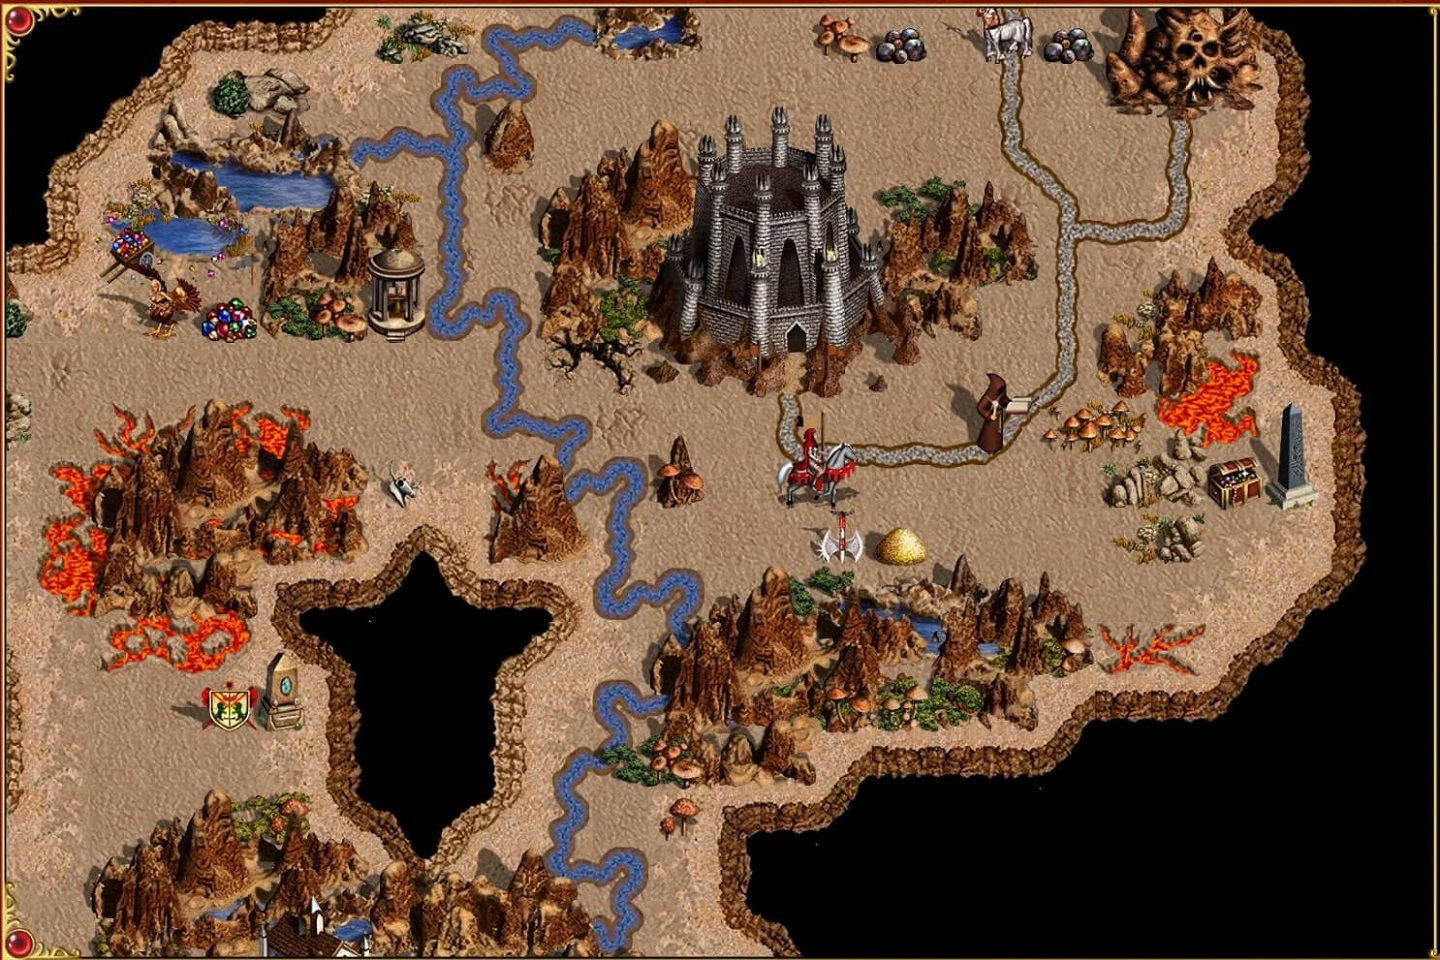
\includegraphics[width=190pt]{images/2d-szinter-HeroesIII.jpg}
  \caption{Felülnézetes színtér\\Heroes III}
  \label{fig:test1}
\end{minipage}%
\begin{minipage}{.5\textwidth}
  \centering
  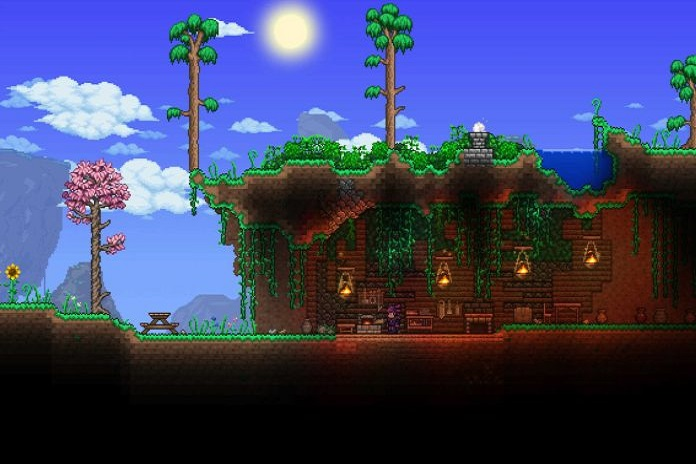
\includegraphics[width=190pt]{images/2d-szinter-Terraria.jpg}
  \caption{Oldalnézetes színtér\\Terraria}
  \label{fig:test2}
\end{minipage}
\caption*{Példa 2D színterekre}
\end{figure}


\chapter{A programról}
Az elkészített program procedurális generálási módszereket tartalmaz. Ezek az eljárások általános felhasználási módokat mutatnak be, nem specifikusan egy alkalmazási területre korlátozódnak.\\
A program használata során több algoritmust vizsgálhat meg a felhasználó, közben különféle paramétereket próbálhat ki. Az eredményként kapott színterek felhasználására a programon belül nincs lehetőség, viszont van, ahol exportálási lehetőség is adott. A kidolgozás során törekedtem arra, hogy a metódusokat sajátos célra is fel tudja bárki használni. 

\section{Tartalom}
Az első dolog amivel találkozik a felhasználó, az egy miniatűr játék-féleség, amit az úgynevezett "Dinosaur Game" ihletett. A Dinosaur Game nevű játékot valószínűleg sokan ismerhetik, hiszen ez a játék jelenik meg a Google Chrome böngészőben, ha nincsen internetelérés.\\
Ez a mini
Ebben a kezdő jelenetben több dolog is történik:
\begin{itemize}
    \item A hátteret egy később bemutatott algoritmus generálja újra és újra.
    \item A képernyőn piros háromszögek csúsznak balra, ahol egy sárga kör található. Ez a sárga kör a felhasználót reprezentálja.
    \item A háromszögek fölött egy megnevezés található. Ez a program során használt jelenetek nevei. Ha nekiütközünk valamelyik háromszögnek, akkor az adott jelentre ugrunk át.
\end{itemize}
A mini-játék során a SPACE billentyűvel tudunk ugrani. Ha nem szeretnénk ezzel a jelenettel bajlódni, akkor az ESC billentyűvel kiléphetünk a fő menübe, ahonnan egyszerűbben navigálhatunk tovább.\\
A jelenetekről részletes útmatás elérhető az a \ref{Utmutato} fejezetben.



\chapter{Algoritmusok}
Az algoritmusok egy fontos tulajdonsága, hogy milyen helyzetben használhatóak, milyen problémákra adnak megoldást. A már említett két eset szerencsére nem különül el egymástól annyira, hogy teljesen új megoldási módszereket kelljen kialakítani.
\section{Kétdimenziós színterek algoritmusai}
Ezen algoritmusok egyszerűbbnek tekinthetőek a színterek kontextusában.


\chapter{Algoritmus általános célokra}
\section{Wave function collapse - Az ötletgazda} \label{WFC-Otlet}
A "WaveFunctionCollapse" nevű algoritmust először githubra publikálta egy felhasználó \footnote{https://github.com/mxgmn/WaveFunctionCollapse}. Az algoritmus nevét a szerző a "hullámfüggvény összeomlásáról" nevezte el, ami egy kvantummechanikai kifejezés. Magának az algoritmusnak nincs szoros kapcsolata ezzel a jelenséggel, de az ihlet onnan jött.
\\Az algoritmus eredeti ötlete, hogy egy inputként megadott bitmap pixeljeit felhasználva generálunk egy, az eredetihez lokálisan hasonló általában nagyobb bitmapet. A módszer azonban nem korlátolt csak bitmapekre: egy adott képet is fel lehet fogni egy bitmapként, amit tetszőlegesen darabolhatunk fel, így lényegében bármilyen képre elvégezhetjük a lépéseket. Ez kifejezetten hasznos több területen is. Egy ilyen felhasználási módszer amit a forrás is említ, hogy az algoritmussal csempézni is lehet a teret.
\\Ezen algoritmus inspirált a sajátos megoldásom elkészítésében. Maga a WFC alapköve az, hogy bármely $NxN$-es blokk a kimenetben fellelhető valamilyen forgatással a bemenetben. Ez a szabály egy elég erős feltétel, illetve magába foglal egyfajta szomszédsági kitételt. A "rejtett" szomszédsági kitétel ihlette az én implementációmat.
\section{Szomszédság alapú blokk generálás - SZABG}
Ahhoz hogy a \ref{WFC-Otlet} pontban említett WFC ihlette algoritmus implementációm egyszerűbben hivatkozható legyen, nevezzük SZABG-nek.
A SZABG eljárás bemenetére csak annyi a kitétel, hogy egy $NxM$-es PNG formátumú kép legyen. Viszont ahhoz, hogy elfogadható kimenetet kaphassunk érdemes az alábbi pontokat szem előtt tartani:
\begin{itemize}
    \item A bemenet legyen egy bittérkép, melyben a pixelek szomsédságát adjuk meg. A pixeleket blokkokként kezelhetjük.
    \item Ha a bemenet nem egy bittérkép, akkor a kép legyen olyan blokkokból készítve, melyek szomszédsága ésszerűen elkészített \textit{(tehát például 16x16 pixelből álló bokor, fa és fű szomszédságának megadása úgy, hogy ezek nem fedik egymást és két blokk között nincs hézag \#KÉP)}.
    \item Használhatunk üres blokkokat is. Üres egy blokk, ha annak alfa csatornája 0. Ezen blokkok nem számítanak bele a szomszédsági kapcsolatokba, és a kimenetben sem szerepelnek. Szerepük a kapcsolatok kialakításának megkönnyítése \#KÉP.
    \item Ha két $NxM$-es blokkban pontosan ugyanazok a pixelek találhatóak, egynek vesszük őket. Ekkor az adott blokkhoz tartozó súly számláló értéke növekszik, aminek eredményeképpen a blokk előfordulásának valószínűsége nagyobb lesz a kimenetben.
    \item A szomszsédságok iránya nem mindegy. Ha egy A blokk csak balról szomszédja egy B blokknak, akkor csak és kizárólag balról érintheti a B blokkot a kimenetben.
    \item A bemenet beolvasása függ a paraméterezéstől, ezért érdemes összehangolni a kettőt.
\end{itemize}

\subsection{Állítható paraméterek}
A SZABG algoritmust futattó program azon paraméterei, melyek a felhasználók által állíthatóak annak futása előtt.
\subsubsection{Bemeneti / kimeneti paraméterek}
Ezen paraméterek határozzák meg, hogy az input képen mekkorák a blokkok, illetve, hogy az output kép nagyságga mekkora legyen.
\begin{table}[H]
\caption{Bemeneti / kimeneti paraméterek}
\label{bemeneti-kimeneti-szabg}
\begin{center}
\begin{tabular}{ |c|c|c| } 
\hline
Paraméter & Leírás & Érték típus \\
 \hline\hline
 Block Width & Egy blokk szélessége & Pozitív egész szám \\ 
 \hline
 Block Height & Egy blokk magassága  & Pozitív egész szám\\ 
  \hline
  Image Width & A generált kép szélessége & Pozitív egész szám \\ 
 \hline
 Image Height & A generált kép magassága  & Pozitív egész szám\\ 
  \hline
\end{tabular}
\end{center}
\end{table}

\paragrafus{Egyéb paraméterek}
Ezek a paraméterek különböző részeit állítját az algoritmusnak, nagyban befolyásolva az eredményt.

\begin{enumerate}
    \item Block Can Neighbor Itself
    \begin{itemize}
        \item Logikai érték. Alapértelmezett értéke: hamis.
        \item Igaz érték esetén globálisan minden blokk bármilyen szomszédja lehet önmagának. A súlyokat és a blokk más blokkokra vett szomszédsági kapcsolatát nem befolyásolja.
        \item Alternatívaként készíthetünk a bemenetre olyan blokkokat, melyek leírják ezt a szomszédságot. Ezzel kiválasztva, hogy pontosan mely cellák legyenek önmaguk szomszédjai. \#KÉP
    \end{itemize}
    \item Wildcard
    \begin{itemize}
        \item CellVariable típusú paraméter. Alapértelmezett értéke: null.
        \item A felhasználó ezt egy vizuális panelen tudja beállítani, ha kevesebb mint 40 különböző blokkot tartalmaz a bemenet.
        \item Egy "joker" blokként fogható fel a beállított blokk. Lényege, hogy bármilyen blokk bármilyen szomszédja lehet. Ha adtunk neki értéket, akkor az algoritmus garantáltan nem akad el.
    \end{itemize}
    \item Block global weight
    \begin{itemize}
        \item Pozitív valós szám. Alapértelmezett értéke a bemenet beolvasása során állítódik.
        \item A felhasználó ezt egy vizuális panelen tudja módosítani minden blokkhoz, ha kevesebb mint 40 különböző blokkot tartalmaz a bemenet.
        \item A paraméter befolyásolja, hogy egy adott blokk milyen globális súllyal rendelkezzen. Minél nagyobb a blokk súlya, annál inkább valószínű, hogy az input egy adott blokkja ilyen legyen (persze az előfordulás nem csak ettől függ). Lokális súlyokat használva nincs hatása.
    \end{itemize}
    \item Cell mode
    \begin{itemize}
        \item Logikai érték. Alapértelmezett értéke: hamis.
        \item Igaz érték esetén a generálás nem ténylegesen egy képet készít, hanem sok kicsit. Pontosabban annyit, amennyi blokkal lefedhető a kívánt kép. Nagyban befolyásolja a program futási idejét, viszont ebben a "cella módban" animálható az algoritmus. Az implementáció során jóval egyszerűbb ezt a módot elkészíteni először.
        \item Hamis érték esetén egy darab tényleges kép objektum generálódik. Virtuális cellákat használva, minden cella erre az egy képre másolja át a tartalmat. Nem animálható, mert a kép pixeleinek beállítasa gyors, viszont annak megjelenítése lassú. Így a futás végén jelenik meg a már kész kép. Jóval gyorsabb futási eredményt okozhat.
    \end{itemize}
    \item{Bias}
    \begin{itemize}
        \item Pozitív valós érték. Alapértelmezett értéke a bemenet beolvasása során állítódik.
        \item Lokális súlyokat használva azt határozza meg, hogy a szomszédos letett cellák mennyire domináns hatással vannak az épp vizsgált cellára nézve. Minél nagyobb az érték, annál inkább lesznek egybefüggő "szigetek" a kimeneten.
    \end{itemize}
\end{enumerate}

\paragrafus{Lokális súlyok és Bias leírása}
A lokális súlyok közvetlenül nem állíthatóak. Csak akkor van hatásuk, ha a "Use local weights" értéke igaz. A bemenet beolvasása közben a program minden blokkra egyesével kialakít egy lokális súly kapcsolatot a szomszédos blokkokkal. Egy kapcsolat a két blokk referenciájából áll, illetve, hogy mekkora ezeknek a súlya. A referenciák, illetve a szomszédsági irány nem releváns. Ha két blokk a bemeneten többször áll egymás mellett, akkor a súly egyel növekszik, új kapcsolat nem jön létre. Minél nagyobb a súlyérték, annál inkább "preferálja" egy blokk azt a szomszédot.\\
Például, ha egy A-B kapcsolatnak a súlya 10, egy A-C kapcsolatnak a súlya 12, akkor a versenyzési fázis során az A blokk a C blokkot adja vissza, mint preferált érték.\\
A versenyeztetési fázis a cellák lerakásakor indul. Lépései:
\begin{enumerate}
    \item \label{lokalis1} A környező cellák először leszűrik, hogy milyen cella kerülhet melléjük.
    \item  A leszűrt cellák visszakerülnek egy ellenőrzésre minden környező cellához, ahol egyenként kiválasztják, hogy melyik cellát preferálják (feltéve, hogy van olyan). Ha több cellát is preferált, akkor véletlenszerűen választódik egy.
    \item A preferált cellák visszakerülnek a \ref{lokalis1} pontban készített listába. Így azok a cellák amelyek preferáltak, többször szerepelnek a listában, mint azok, amelyek nem.
    \item A cellákat csoportosítjuk az előfordulások számának függvényében, új súlyokat létrehozva ezzel. A legnagyobb súlyú celláknak megszorozzuk a súlyát a Bias paraméter értékével.
    \item Az így keletkezett opciókból a súlyokat figyelembe véve véletlenszerűen választunk (a nagyobb súlyú celláknak nagyobb esélye van a kiválasztásra).
\end{enumerate}
A versenyeztetés során az opciók száma nem csökken, illetve a választási valószínűségük sem lesz 0. Ez garantálja azt, hogy változatos lesz a végeredmény, még viszonylag magas Bias érték mellett is.



\begin{table}[htbp]
\caption{Egyéb paraméterek összefoglalása}
\begin{center}
\begin{tabular}{ |c|c|c| } 
\hline
Paraméter & Leírás & Érték típus \\
 \hline\hline
  \makecell{Block Can \\ Neighbor Itself} & \makecell{Ha igaz, akkor minden blokk 
 \\szomszédja önmagának minden irányból} & Logikai érték \\
 \hline
 Wildcard &\makecell{ Olyan blokk, ami bármilyen blokk \\ bármilyen szomszédja lehet} & CellVariable \\ 
 \hline
 Block global weight & Egy blokk globális súlya  & Pozitív valós szám\\ 
  \hline
  Animate & \makecell{A generálás animálódjon-e \\ (csak cella módban!)} & Logikai érték \\
 \hline
  Cell mode & Cella mód ki/be kapcsolása. & Logikai érték \\
 \hline
  Use Local weights & \makecell{Lokális vagy globális súlyokat \\ használjon-e az algoritmus.} & Logikai érték \\
 \hline
 Bias & \makecell{Lokális súlyok esetén mennyire legyen \\ domináns a letett cellák befolyása. \\ } & Pozitív valós érték \\
 \hline
\end{tabular}
\end{center}
\end{table}



\subsection{Az algoritmus lépései}
A paraméterek áttekintése után, vessünk egy pillantást a lépésekre. Önmagában nem feltétlenül tűnik bonyolultnak az eljárás elképzelése: olvassunk be blokkokat, majd tegyük le őket kvázi véletlenül. Ennél azért bonyolultabb a tényleges működés, hiszen szomszédsági kapcsolatokat kell kialakítanunk. Ez növeli a komplexitást, illetve elválasztja a teljesen véletlen generálástól a SZABG-t.
\begin{enumerate}
    \item Beolvassuk az inputot.
    \item Elkészítjuk az input alapján a blokkokat, a \ref{bemeneti-kimeneti-szabg} paramétereknek megfelelően. A blokkokhoz globális és szükségszerűen lokális súlyokat számítunk.
    \item Minden blokkhoz hozzárendeljük a pozícióját, illetve meghatározzuk, mely blokkok szomszédosak egymással.\\
    A szomszédokat az alábbiként definiáljuk:
    \begin{itemize}
        \item Ha egy blokk koordinátái: $(x,y)$, akkor szomszédjainak koordinátái: \\
        $(x-1,y), (x+1,y), (x,y-1),(x,y+1)$
        \item A blokkokat egy tóruszon képzeljük el. Ez azt jelenti, hogy ha összesen $NXK$ blokk van, akkor az $(1,j), (j = 1,2,3...k)$ koordinátájú blokkok bal szomszédja az $(n,j), (j = 1,2,3...k)$ koordinátákon helyezkednek el. Ez a kapcsolat minden szélső blokkra hasonlóan igaz.
    \end{itemize}
    \item Lefedjük az output képet üres \textit{cellákkal}, amik egy-egy blokkot fognak megjeleníteni.
    \item Kiválasztjuk, hogy melyik üres cellát szeretnénk feltölteni. Ez a kiválasztás az alábbi eljárások egyikével történik:
    \begin{itemize}
    \label{item:modszer}
        \item Horizontálisan / vertikálisan, azaz elindulunk egy soron / oszlopon és folytonosan választjuk a cellákat.
        \item Véletlenszerűen.
        \item Kiszámítjuk minden cella \textit{entrópiáját}, majd mindig a legalacsonyabb entrópiájú cellát választjuk. A \textbf{cella entrópiája} az a mennyiség, amely megadja, hogy mennyire "bonyolult" meghatározni, hogy milyen blokkot fog tartalmazni a cella. Egy cella blokkját annál bonyolultabb meghatározni, minél több közel egyenlő valószínűségű opció közül lehet választani.\\
        Legyen a cellák halmaza $C$, a cellára letehető blokkok halmaza $B$. Egy $c\in C$ cella entrópiáját az alábbi képlettel számolhatjuk: $$E(c) = \sum_{i=1}^{n}P(b_i) * \log{1/P(b_i)}$$ ahol $n$ a $B$ halmaz elemszáma, $b_i\in B$, $P(b_i)$ pedig az adott blokk \textit{globális elhelyezési valószínűsége}. Egy $b\in B$ blokk \textbf{globális elhelyezési valószínűsége:} $$P(b) = \frac{S_b}{S_B}$$\\
        Ahol $S_b$ a $b$ blokk globális súlya, $S_B$ pedig az összes, a cellára letehető blokk globális súlyának összege.
    \end{itemize}
    \item Addig ismételjük a 3. ponttól az algoritmust, míg le nem fedtuk az outputot, vagy el nem akadtunk.\\
    Az elakadás egy probléma ami akkor jelenik meg, ha olyan üres cellához érünk, melynek szomszédjai kizárják egymást. Ekkor az algoritmust újrakezdjük, vagy leállunk. Egy ilyen elakadási helyzetre példa a \#KÉP ábra.\\
    Elakadás nem lehetséges, ha van olyan blokk, amely bármilyen másik blokk szomszédja lehet.
\end{enumerate}

\newpage

\subsection{Felhasználás}
Az algoritmus első ránézésre csak textúrákat képes generálni, viszont ez nem feltétlenül igaz. Képzeljünk el egy bemenetet, ahol háromféle blokk van: barna, zöld, sárga. Ezek a blokkokat később felfoghatjuk földként, fűként és virággként. Ha egy megfelelő inputot megadunk a programnak, legenerálhatjuk egy mező felülnézeti térképét. A letett blokkok színét és helyzetét felhasználva ebből egy háromdimenziós színteret is előállíthatunk.\\
Egy kétdimenziós színtér esetén a generálás már-már kész eredményt is adhat. Nem szabad elsiklani afölött a tény fölött, hogy a színtér készítése az eljárás végével nem kell, hogy megálljon. Az eredményt tetszőleges módon lehet exportálni és importálni, a felhasználás során az adatokat átrendezhetjük.

\chapter{Égitestek elhelyezése - Űrbéli játékhoz}
Ez a fejezet egy olyan algoritmusról szól, mely követi az alapjait egy már létező videójáték generálási szabályainak. Ez névszerint a Galactic Civilizations III, űrben játszódó, körökre osztott videójáték pálya generálása.\\
Nem teljesen ugyanolyan szabályrendszert alkaztam, mint az említett játékban, mivel a pontos szabályai, lépései és implementációja nem publikusan elérhetőek, illetve csak az alapötlet átvétele volt a célom. A módszerem jóval egyszerűbb, illetve nem annyira kifinomult, viszont egy szerintem érdekes problémát tárgyal.\\
A probléma a következő: hogyan helyezhetünk el úgy pontokat, hogy azok játékmenet szempontjából igazságos és változatos legyenek? Ezt egy kicsit másképp megfogalmazva: hogyan helyezhetünk el úgy pontokat, hogy azok véletlenszerűnek tűnjenek, de legyen közöttük egy minimális távolság? A távolság megkötés azért kell, mert ekkor a pontok \textit{esztétikusan} fedik le a síkot. Esztétika alatt értendő az, hogy két véletlenszerűen megvizsgált területen, nagyjából azonos mennyiségű pont van, függetlenül a területek megválasztásától. A két feltétel ellentmondásos, így a köztes megoldás megtalálása a cél.

\section{Az eljárás alapjai}
A módszer során pontokat teszünk le egy meghatározott területre, ahol minden pont egy-egy elem a Galactic Civilizations III játékból. Az elemek a következők: csillagok, fekete lyukak, bolygók, nyersanyagok. A kitételek ezekre a pontokra a következők:
\begin{itemize}
    \item Minden pont között van legalább $d_1$ egységnyi távolság.
    \item Csillagok és fekete lyukak között van legalább $d_2$ egységnyi távolság úgy, hogy $d_1 < d_2$.
    \item A fekete lyukak két zónát határoznak meg. Az elsó zóna egy $b_1$ sugarú kör, ezen a körön belül nem lehet más pont. A második zóna egy $b_2$ sugarú kör, ezen a körön belül nem lehet másik fekete lyuk ($b_1 < b_2$). A körök középpontjának az adott fekete lyukat vesszük.
    \item A csillagok $c$ sugarú környezetében helyezkedhetnek el a bolygók.
    \item A pontokat a már említett esztétika szerint helyezzük el.
\end{itemize}
Az algoritmus során a pontok generálási sorrendje: csillagok, fekete lyukak, bolygók, nyersanyagok. A sorrend nem szükségszerű, de érdemes betartani.

\section{Állítható paraméterek}
Azon paraméterek, amik a felhasználó által állíthatóak a jelenet során.
\begin{enumerate}
    \item \label{gc-allithato-1} World height / width: ezek a paraméterek határozzák meg azt a területet, amire először generál az algoritmus. Értékük egy pozitív egész szám. Alapértelmezett értékük : 16x9.
    \item Max number of stars: a paraméter azt határozza meg, hogy maximum mennyi csillagot tehet le az eljárás. A végeredményben szereplő csillagok száma ennél általában kevesebb. Pozitív egész szám. Alapértelmezett értéke: 30.
    \item Max number of black holes: hasonlóan a csillagokhoz, maximálisan ennyi fekete lyuk jelenhet meg a síkon. Pozitív egész szám. Alapértelmezett értéke: 10.
    \item Resource density: a fennmaradt üres helyekre mekkora eséllyel kerüljön nyersanyag. Az értéke pozitív valós szám, 0 és 1 között. Alapértelmezett értéke: 0,45.
    \item Spacing: a módszer először az \ref{gc-allithato-1}. pontban meghatározott értékek szerinti területre teszi le a pontokat. Ezzel a paraméterrel lehet skálázni a pontok koordinátáit, azaz a pontok koordinátái ezen értékkel szorzódnak. Pozitív valós érték. Alapértelmezett értéke: 3.
    \item Position noise: az elhelyezés során a pontokat négyzetrács pontokra tesszük le, ez a paraméter azt határozza meg, hogy az adott pontot a rácsponttól maximum mekkora távolságra tolhatjuk el valemely irányba. Ez az érték biztosítja a változatosabb, kevésbé kiszámítható elhelyezést. Az eltolás még a skálázás előtt történik. Pozitív valós szám. Alapértelmezett értéke: 0,5.
    \item Planet density: a csillagok köré generáljuk a bolygókat. Ezt összesen 8 helyre próbáljuk meg, minden csillag esetén. Ez a paraméter határozza meg, hogy mekkora eséllyel kerül az adott helyre bolygó. Pozitív valós szám. Alapértelmezett értéke: 0.2.
    \item Max number of planets/star: a csillagok köré maximum hány bolygó kerülhet. Pozitív egész szám, maximum 8. Alapértelmezett értéke 4. 
\end{enumerate}

\newpage
\begin{table}[htbp]
\caption{Paraméterek összefogalása}
\begin{center}
\begin{tabular}{ |c|c|c| } 
\hline
Paraméter & Leírás & Érték típus \\
 \hline\hline
  World height & A generálási terület magassága & Pozitív egész érték \\
 \hline
 World width & A generálási terület szélessége & Pozitív egész érték \\
 \hline
 \makecell{Max number of\\ stars} & Maximum ennyi csillag generálódhat  & Pozitív egész érték \\ 
  \hline
  \makecell{ Max number of \\ black holes} & Maximum ennyi fekete lyuk generálódhat  & Pozitív egész érték \\ 
 \hline
  Resource density & \makecell{A fennmaradt üres helyeken mekkora \\ valószínűséggel teszünk nyersanyagot} & \makecell{Pozitív valós érték \\0 és 1 között }\\
 \hline
  Spacing & A terület felskálázására szolgál & Pozitív valós érték \\
 \hline
 Position noise & \makecell{Rácspontoktól vett maximum távolság \\ valamely irányba} & Pozitív valós érték \\
 \hline
  Planet density & \makecell{A csillagok mellett lévő pontokban\\ mekkora eséllyel generálódhat bolygó.} & \makecell{Pozitív valós érték \\0 és 1 között}\\
 \hline
\makecell{Max number of\\ planets/star} & \makecell{Maximum hány bolygó kerülhet \\ a csillagok mellé} & \makecell{Pozitív egész érték \\ maximum 8}\\
 \hline
\end{tabular}
\end{center}
\end{table}

\newpage
\section{Az algoritmus leírása}
Az eredeti problémára nem egyszerű olyan megoldást adni, ami ésszerű és belátható időn belül lefut. A nehézség abban rejlik, hogy milyen módon tudjuk biztosítani a pontok közötti távolság megszorítását, találomra lehelyezett pontok esetén. Ha véletlenszerűen kezdünk el pontokat letenni a síkra, majd valamilyen séma alapján javítjuk vagy elvetjük a pontokat, könnyen eshetünk abba a csapdába, hogy túl lassú, vagy kiszámíthatatlan programot készítünk. Így érdemes a másik irányból megközelíteni a problémát: generáljunk először olyan pontokat, amik biztosan a megadott minimális távolságra vannak egymástól, majd ezeket a pozíciókat finomíthatjuk, hogy a véletlenszerűség is megjelenjen.\\
A megadott területet egy négyzetrácsként képzeljük el. Ha a terület $NxK$ nagyságú, akkor egy $NxK$-s négyzetrácsra tesszük az összes pontot. Miután megjelöltünk egy pontot adott égitestként, a \textit{Position noise} paraméter alapján eltoljuk azt valamely irányba. Az, hogy a különböző fajtájú komponensek letevése között milyen sorrendet választunk, megváltoztathatja a végeredményt. Az előbb generált elemek határozzák meg a később letett elemek mennyiségét és pozícióját, ezt érdemes szem előtt tartani.\\
Kezdjünk a csillagok lehelyezésével. Az $NxK$ darab pont közül kiválasztunk annyit, amennyi a \textit{Max number of stars} paraméter értéke, majd ezeket megjelöljük csillagként. Ahhoz, hogy ne egy valamilyen minta szerint válasszuk a pontokat, összekeverjük őket.\\
A csillagok lehelyezése után fennmaradt üres helyekre tegyünk fekete lyukakat. A pontokat ugyanúgy összekeverjük. Egy fekete lyuk lehelyezése után végigmegyünk a környező rácspontokon, és az első zónába eső pontokat megjelöljük üresnek. A második zónába eső pontokat pedig megjelöljük olyan pontoknak, amik nem lehetnek fekete lyukak. Az üres pontokon addig megyünk végig, amíg a megfelelő mennyiségű fekete lyukat meg nem jelöltük, vagy az összes üres ponton végig nem mentünk.\\
Az így fennmaradt szabad helyekre a nyersanyagokat tesszük. Összekeverjük az összes pontot, majd azon pontokra, amelyek még szabadok, eldöntjük, hogy teszünk nyersanyagot vagy sem. Ezt a \textit{Resource density} paraméter befolyásolja. Minél nagyobb az értéke, annál nagyobb eséllyel lesz a pont megjelölve nyersanyagként (1-es érték esetén biztosan).\\
Végezetül a csillagok köré lehelyezzük a bolygókat. A bolygók egy kicsit megnehezítik a helyzetet, mert nem kerülhetnek a fekete lyukak első zonájába. A feltételt biztosíthatjuk azzal, hogy a bolygók generálása után elvetjük azokat, amelyek a szabályt sértik, vagy a skálázással érjük el a kívánt végeredményt. Most válasszuk a második megoldást. Ez esetben nincs szükség egyéb megszorításra a bolygók terén, csak arra, hogy mekkora távolságra legyenek a csillagoktól. Ezt elérhetjük újból a négyzetrácsos módszerrel. Egy $3x3$-as négyzetrácsot készítünk, melynek középső pontja a vizsgált csillag. A többi nyolc ponton végigmegyünk, majd mindegyik pontra eldöntjük, hogy üres maradjon, vagy bolygót tegyünk rá. A \textit{Planet density} és a \textit{Max number of planets/star} paraméterek döntik el, hogy adott pontba mekkora eséllyel, illetve, hogy összesen mennyi bolygó kerülhet a csillag mellé.
\chapter{Útmutató}
\label{Utmutato}
A program elején egy jól ismert mini-játék fogad az úgynevezett "Dino game". Az implementációm egy jóval egyszerűbb verziója az eredeti játéknak, egy játékos menüként fogható fel.
\begin{itemize}
    \label{item:dino-runner-utmutato}
        \item Ugrani a "SPACE" billentyűvel lehet
        \item Piros háromszögek jönnek elő jobbról, ezeknek ha neki ütközünk akkor a háromszög tetején látható scene-re irányítódunk át.
\end{itemize}
\textbf{Fontos:} minden scene rendelkezik egy felugró menüvel, ezt az "ESCAPE" billentyűvel érhetjük el. Innen a "Main menu" gombot lenyomva áttérhetünk egy hagyományosabb kezdő menüre.\\
Az alábbi scene-ek érhetőek el a menüből:\\
GC\\
WFC / WFCSelectorScene\\
\textit{SubwaySurfer}
\section{GC}
Irányítás:
\begin{itemize}
    \label{item:GC-iranyitas}
        \item Nagyítani-kicsinyíteni a görgővel lehet.
        \item A kamerát a WASD és a nyilak segítségével mozgathatjuk.
\end{itemize}
Használat:
\begin{itemize}
    \label{item:GC-hasznalat}
        \item A "Run algorithm" gombbal generálhatunk új világot. Ez paraméterezés nélkül is működik, előre beállított értékékkel.
        \item World dimensions: 
        \begin{itemize}
            \item Width: a világ négyzetrácsának vízszintes nagysága
            \item Height: a világ négyzetrácsának függőleges nagysága
        \end{itemize}
        \item Max number of stars: megadható hogy maximum hány csillag generálódjon a térben. A végleges száma a csillagoknak ettől eltérő lehet (kevesebb). Maximum $$Width * Height$$ darab csillag generálható.
        \item Max number of black holes: megadható hogy maximum hány fekete lyuk generálódjon a térben. A végleges száma a feketelyukaknak ettől eltérő lehet (kevesebb). Maximum $$Width * Height - Csillagok$$ feketelyuk generálható.
        \item Resource density: megadható milyen sűrűen legyenek elhelyezve "relikviák". 0-1 közötti érték, az üresen maradt helyek száma határozza meg a generálást.
        \item Spacing: a világ négyzetrácsainak nagyságát lehet állítani vele. A generálás egységnyi nagyságú négyzetrácsokon történik, aztán kerül sor a transzformációra.
        \item Position noise: a négyzetrácsok közepétől mekkora sugarú körben vándorolhatnak el az égitestek. A változásra még a "Spacing" paraméter hatása elött kerül sor.
\end{itemize}
\section{WFC / WFCSelectorScene}
Használat:
\begin{itemize}
    \label{item:WFC-hasznalat}
        \item A program beolvassa a /Szakdolgozat2D\_Data/StreamingAssetsPath/input \\
        mappában lévő png kiterjesztésű fájlokat, ezen képeket használhatjuk fel a generálásra. Valamely képre kattintva, majd a felugró ablakon a "load" gombot lenyomva haladhatunk tovább.
        \item Cell can neighbor itself: ezen beállítással módosítható, hogy a képből generált cellák szomszédjai lehetnek-e saját maguknak mindenféleképpen, vagy csak akkor, ha az a referencia képen is látható.
        \item Continous block picking: ezen beállítással módosítható, hogy a beolvasás során a blokkok takarhatják-e egymást vagy sem. Igaz érték esetén minden NxM-es blokkot beolvas a program, hamis esetén pedig úgy, mintha dominók lennének.
        \item Block dimensions: 
        \begin{itemize}
            \item Width: a blokkok szélessége.
            \item Height: a blokkok magassága.
        \end{itemize}
        \item Image size: mekkora a referencia képünk nagysága pixelekben mérve.
        \item Potential block count: ha minden blokk különböző lenne, akkor mennyi blokk képződne az eljárás során.
        \item Generate: a gomb lenyomásával legenerálódnak a blokkok. A gomb lenyomása után két gomb válik láthatóvá:
        \begin{itemize}
            \item Check blocks: ha kevesebb mint 40 blokk generálódott, akkor megtekinthetőek a gomb lenyomásával.  A feulgró ablakban láthatóak a blokkok, illetve alattuk az, hogy mekkora súllya van egy blokknak. Ez a súly változtatható, illetve negatív érték esetén a blokk bellítható "wildcard" blokknak (ilyen esetben a blokk súlya nem változik).
            \item Next: a következő paraméterezésre léphetünk át.
        \end{itemize}
\end{itemize}
Next gomb lenyomása után:
\begin{itemize}
    \label{item:WFC-hasznalat3}
        \item Animate the algorithm: csak cella módban működik. A generálás blokkról-blokkra láthatóva válik. A generálás során kikapcsolható.
        \item Cell mode: cella módban, vagy egyszerűsített módban generáljon az algoritmus. A cella mód egyenként fog kép objektumokat generálni, az egyszerűsített mód pedig egy képet generál. Nagy méretű textűra generálás esetén ajánlott az egyszerűsített mód.
        \item Use local weights: a generálás során lokális vagy globális súlyokat használjon a program.
        \item Block dimensions: a szélességnek és magasságnak oszhatónak kell lennie a blokk szélességével / magasságával.
        \begin{itemize}
            \item Width: a generált kép szélessége.
            \item Height: a generált kép magassága.
        \end{itemize}
        \item Image size: mekkora lesz a tényleges képméret, képpontokban megadva.
        \item Model: kiválasztható melyik bejárási model szerint generáljon a program.
        \begin{itemize}
            \item HORIZONTAL / VERTICAL: vízszintes / függőleges bejárási irány.
            \item RANDOM: véletlenszerű bejárási irány. Magasabb az esélye hogy a generálás elakad, ha sok a megszorító szomszédsági reláció.
            \item SHANNON\_MODEL: Shannon-entrópiát használó bejárás. Lassabb mint a többi.
        \end{itemize}
        \item Run algorithm: a képgenerálás lefuttatása. A futtatás után a paraméterek újra változtathatóak. A blokkok változtatása csak a menübe kilépve érhető el újra.
\end{itemize}
\section{SubwaySurfer}
Ez a scene csak a "runner" scene-ből érhető el.
\begin{itemize}
    \label{item:SubwaySurfer-hasznalat}
        \item Mozogni a nyilakkal, illetve a WASD billentyűkkel lehet. Ütközés esetén az "ESCAPE" lenyomása után a "runner" menüpontból érhető el a scene.
\end{itemize} 

%biblatex verzió
%a bibintoc heading stílussal megjelenik a tartalomjegyzékben, title-lel a megjelenő címsor szövege módosítható
\printbibliography[heading=bibintoc,%
title=Források]
%sima bibtex verzió
%\bibliographystyle{plain}
%\bibliography{dolgozat.bib}

\include{cover/hasznalati}

\end{document}
